% BLOQUE A -- Técnicas de elicitación (Basurto). Parte 1: introducción y entrevista.
% Contenido propio.

% ---------- Diapositiva 1 ----------
\begin{frame}{Por qué importa elicitar}
  \small
  \begin{itemize}
    \item Elicitar es descubrir qué necesitan los stakeholders y volver explícito lo implícito \cite[p.~34]{ireb2026}.
    \item Kano \cite[p.~34]{ireb2026}:
    \begin{itemize}
      \item \textbf{Satisfiers:} conocimiento consciente. Lo piden.
      \item \textbf{Dissatisfiers:} subconsciente. Se da por obvio.
      \item \textbf{Delighters:} inconsciente. Sorprende al descubrirlo.
    \end{itemize}
    \item \textbf{Idea propia:} la técnica decide qué conocimiento sale.
  \end{itemize}
\end{frame}

\begin{frame}{Qué conocimiento alcanza cada técnica}
  \small
  \begin{itemize}
    \item Preguntar, colaborar y observar: sobre todo satisfiers y dissatisfiers \cite[p.~34]{ireb2026}.
    \item Técnicas creativas, como el prototipado: delighters \cite[pp.~34--35]{ireb2026}.
    \item \textbf{Mi mapeo (interpretación propia):}
    \begin{itemize}
      \item Entrevista: lo consciente y parte de lo subconsciente.
      \item Taller: consciente y subconsciente, con acuerdos.
      \item Prototipado: lo inconsciente, porque reaccionan al ver algo.
    \end{itemize}
  \end{itemize}
\end{frame}

% ---------- Entrevista ----------
\begin{frame}{Entrevista}
  \small
  \textbf{Qué es:} el analista pregunta a un stakeholder para obtener requisitos \cite[Sec.~19.2, pp.~245--255]{pohl2025}

  \vspace{4pt}
  \centering
  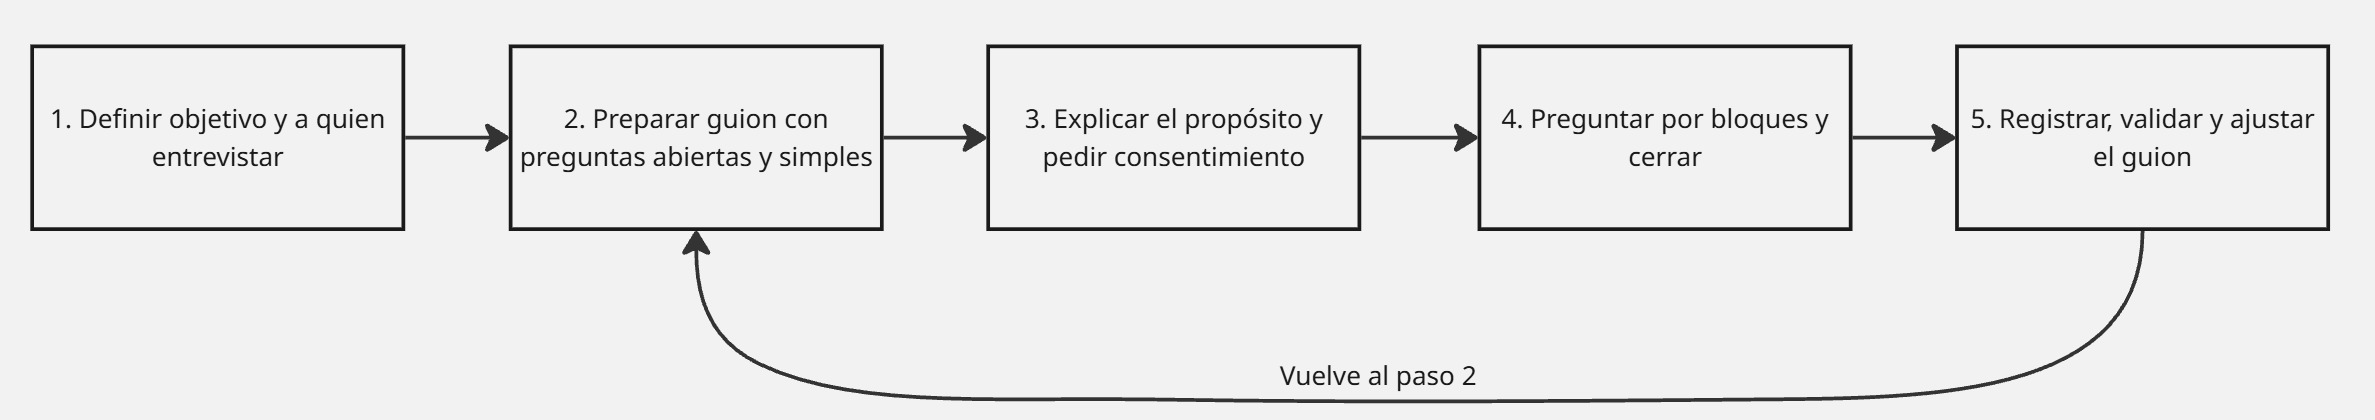
\includegraphics[width=\textwidth]{figuras/flujo-entrevista.jpg}

  \raggedright
  \vspace{10pt}
  \textbf{Cuándo:} pocos stakeholders clave y detalle individual \cite[Sec.~19.2, pp.~245--255]{pohl2025}
\end{frame}

\begin{frame}{Entrevista: ventajas, limitaciones y ejemplo propio}
  \small
  \begin{columns}[T]
    \begin{column}{0.48\textwidth}
      \textbf{Ventajas}
      \begin{itemize}
        \item Más fácil de agendar que un taller grande \cite[Cap.~7, pp.~121--122]{wiegers2013}
        \item Permite repreguntar en el momento.
      \end{itemize}
      \textbf{Limitaciones}
      \begin{itemize}
        \item Solo sale lo que el entrevistado sabe decir.
        \item Preguntas inductivas o dobles sesgan.
      \end{itemize}
    \end{column}
    \begin{column}{0.48\textwidth}
      \textbf{Ejemplo propio (GA-TL-02, P3)}
      \begin{itemize}
        \item \textbf{Original:} «¿Qué problemas o atrasos les da trabajar con las hojas impresas de inscripción?»
        \item \textbf{Defecto:} inductiva y doble.
        \item \textbf{Corregida:} «¿Cómo es su experiencia trabajando con las hojas impresas de inscripción?»
      \end{itemize}
    \end{column}
  \end{columns}
\end{frame}
